\section{Exploring Interleaving Space}
\label{s:design}

\cut{
\begin{itemize}
\item our approach in one sentence: defining the universal set $U$
  using a coverage metric, and directing execution to consume the
  universal set
\item coverage
  \begin{itemize}
  \item rationale:
  \item challenges:
  \item solution:
  \end{itemize}
\item interleaving mutation
  \begin{itemize}
  \item rationale:
  \item challenges:
  \item solution:
  \end{itemize}
\item what do we do to explore the interleaving space?
  \begin{itemize}
  \item We take an interleaving (= a totally ordered instruction sequence as an input)
  \item mutate an interleaving to generate another interleaving
  \item how?
    \begin{itemize}
    \item collect {C1, C2, ...} from the interleaving
    \item infer $U$, the universal set of coverage
    \item consume $U$ until it is empty
    \end{itemize}
  \end{itemize}
\item an intuition for a coverage
  \begin{itemize}
    \item observations
      \begin{itemize}
      \item interleavings are directed acyclic graph
      \item multiple pairs of conflicting accesses are a subgraph of an interleaving
      \end{itemize}
  \item we represent a coverage using a graph (?)
  \end{itemize}

\item an intuition for an interleaving mutation
  \begin{itemize}
  \item two observatrions
    \begin{itemize}
      \item many coverages can be executed together
      \item we can infer what coverages should be further tested
      \end{itemize}
  \item step 1: collect coverage
  \item step 2: inference of coverages to test
  \item step 3: collect coverages that can be tested together
  \item step 4: generate an interleaving to test
  \end{itemize}
\end{itemize}
}


In this section, we describe our approach to explore the interleaving
space.
%
We first provide the overview of our
approach~(\autoref{ss:overview}). Then, we illustrate our coverage
metric in the concurrency dimension~(\autoref{ss:coverage}), and the
instruction scheduling algorithm to quickly saturate the
coverage~(\autoref{ss:scheduler}).

\subsection{Approach Overview}
\label{ss:overview}

\begin{figure*}[ht]
  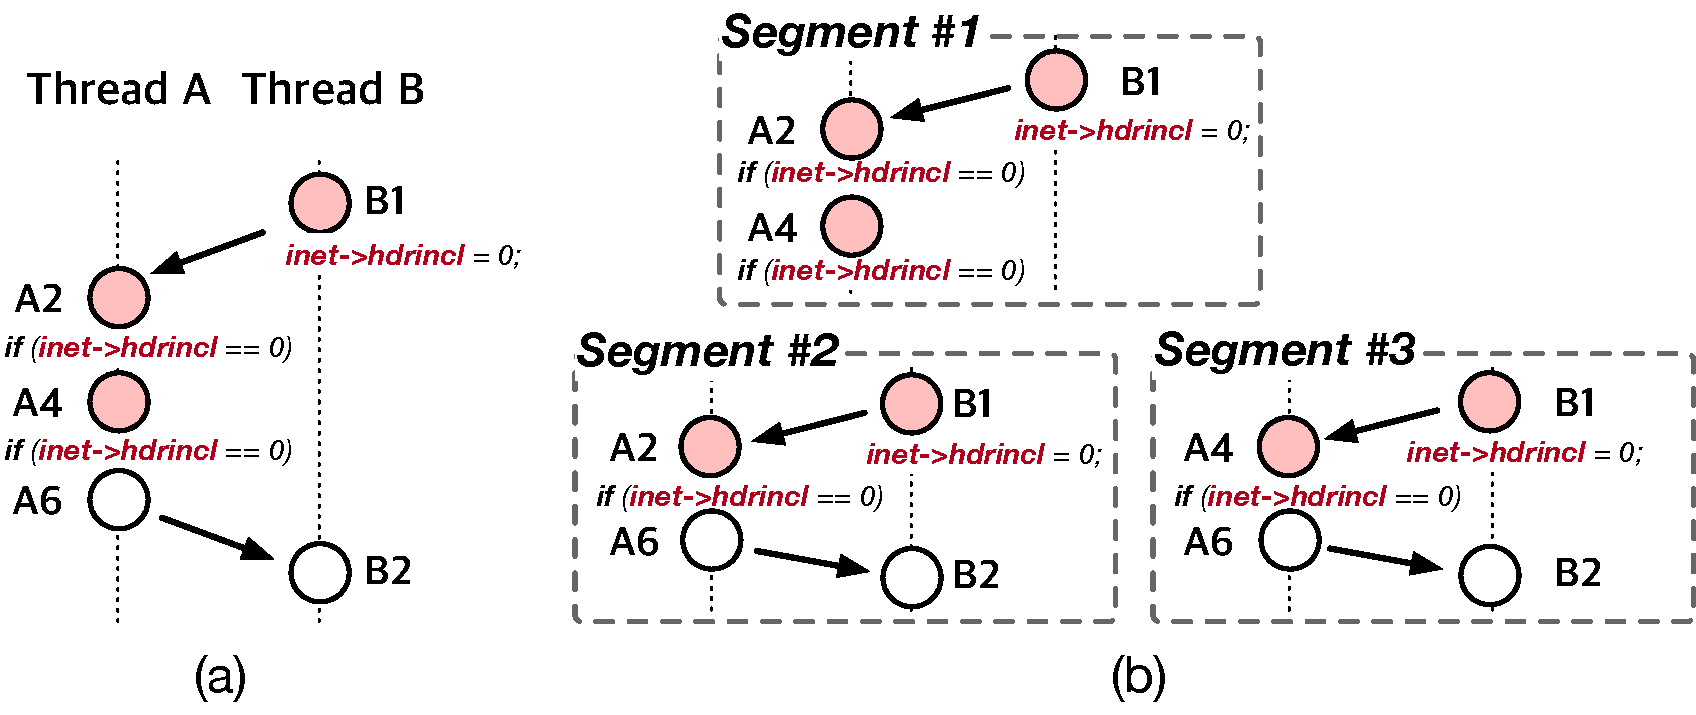
\includegraphics[width=0.9\linewidth]{fig/intuition.pdf}
  \caption{Approach overview to explore the interleaving
    space. \dr{TODO: describe who conflicts with who}}
  \label{fig:overview}
\end{figure*}

Our approach to explore the interleaving space assumes that a
concurrent job (\eg, a set of syscalls) and an initial interleaving
(\ie, a seed interleaving) of the concurrent job are given as an
input. We also assume that all memory access operations in a seed
interleaving are totally ordered.

With the given input, we deal with the interleaving as a subject of
mutation. In other words, from the given seed interleaving, we first
track coverage in the concurrency dimension (shortly, concurrency
coverage) that tracks conjunctions of scheduling constraints. After
that, we generate other interleavings by rescheduling instructions for
finding new concurrency coverage.
%
As a result, we generate various interleavings of the given concurrent
job that disclose different concurrency coverage.
%
\dr{This does not mention the race-steered control flow.}
%
\dr{what about sequential coverage and mutations?}

\PP{Biconflict coverage}
%
We design a concurrency coverage metric to address \textit{an emprical
  aspects of race conditions}.
%
To recap, as described in \autoref{s:motivation}, most race conditions
manifest if at most \textit{two} scheduling constraints on at most
\textit{four} memory access operations are fulfilled.
%
Furthermore, considering a thread (thread~A) may affect execution of
another thread (thread~B) only if thread~B reads a value written by
thread~A, scheduling constraints should be established on a pair of
conflicting memory access operations.

To reflect this nature of race conditions, we propose a novel coverage
metric, called biconflict coverage, that tracks the execution order of
two pairs of conflicting memory access operations.
%
As biconflict coverage tracks the sufficient condition for most race
conditions to manifest, if we find all biconflict coverage in the
given concurrent job, we have a strong confidence that the concurrent
job does not reveal a race condition.

Throughout the rest of this paper, a term ``scheduling constraint
pair'' denotes a conjunction of two scheduling constraints, and a term
``offending scheduling constraint pair'' denotes a scheduling
constraint pair that causes a race condition.  For example,
$(\texttt{A1} \rightarrow \texttt{B1}) \wedge (\texttt{B4} \rightarrow
\texttt{A2})$ is an offending scheduling constraint pair of the race
condition in \autoref{fig:cve-2019-6974}.

\PP{Challenge}
%
% \dr{
% \begin{itemize}
% \item rationale: we need to test muliple pairs of conflicting accesse
% \item challenges: the search space is too large
% \item solution: infer the universal set $U$ and direct the interleaving mutation towards undisclosed coverage
% \end{itemize}
% }
%
One could argue that tracking biconflict coverage is intractable since
the size of the search space is too large.
%
If two threads conflict on $N$ pairs of memory accesses, the number of
scheduling constraint pairs is propotional to $N^2$, which is possibly
too large to test one-by-one.

However, it is worth noting that many scheduling constraint pairs are
not exclusive.
%
When a concurrent job is executed conforming with an interleaving, we
can observe that the interleaving obeys many scheduling constraint
pairs simultaneously.
%
\dr{example}

Our intuition to explore the interleaivng space is based on the
observation.
%
Let us suppose we know which scheduling constraint pairs are
undisclosed. Among undisclosed scheduling constraint pairs, we can
select scheduling constraint pairs that are not exclusive with each
other, and schedule instructions to experience the selected
scheduling constraint pairs.
%
\dr{TODO: define univeral set U of scheduling constraints}


\PP{Overall steps}
%
\dr{Assume $U$ is a universal set of all scheduling constraint pairs
  of the given concurrent job}
%
Let us suppose we have a concurrent job consisting of \texttt{mmap()}
and \texttt{ioctl(TRANSACTION)} in \autoref{fig:cve-2019-6974}, and
\autoref{fig:overview}-(a) represents an initial interleaving of the
concurrent job.
%
As described the figure, the initial interleaving is provided with an
execution order of
$\texttt{A1} \rightarrow \texttt{A2} \rightarrow \texttt{B1}
\rightarrow \texttt{B4} \rightarrow \texttt{B5} \rightarrow
\texttt{A3}$.
%
In the given interleaving, the race condition does not manifest since
\texttt{A2} is executed before \texttt{B4}, which violates the
offending scheduling constraint pair,
$(\texttt{A1} \rightarrow \texttt{B1}) \wedge (\texttt{B4} \rightarrow
\texttt{A2})$.

With the given input, the first step is to track biconflict coverage.
In the given interleaving of \autoref{fig:overview}-(a), three
scheduling constraints (\ie, $\texttt{A1} \rightarrow \texttt{B1}$,
$\texttt{A2} \rightarrow \texttt{B4}$, and
$\texttt{B5} \rightarrow \texttt{A3}$) are fulfilled.
%
By pairing these scheduling constraints, we construct three scheduling
contraint pairs, namely
$(\texttt{A1} \rightarrow \texttt{B1}) \wedge (\texttt{A2} \rightarrow
\texttt{B4})$,
$(\texttt{A1} \rightarrow \texttt{B1}) \wedge (\texttt{B5} \rightarrow
\texttt{A3})$, and
$(\texttt{A2} \rightarrow \texttt{B4}) \wedge (\texttt{B5} \rightarrow
\texttt{A3})$.
%
\autoref{fig:overview}-(b) represents the three scheduling constraint
pairs.
%
Assuming we initially have empty biconflict coverage, the three
scheduling constraint pairs are recorded as new coverage of the given
interleaivng.



After tracking biconflict coverage from the given interleaving, we
determine whether the interleaving is worth further mutation.
%
To this end, we adopt a strategy to \textit{predict coverage that is
  likley found when the interleaving is mutated}.
%
Taking the example of \autoref{fig:overview}-(c), we can derive a
scheduling constraint pair \texttt{Segment 1'} from \texttt{Segment 1}
by flipping the execution order of
$\texttt{A2} \rightarrow \texttt{B4}$ to
$\texttt{B4} \rightarrow \texttt{A2}$.
%
Similarily, \texttt{Segment 2'} and \texttt{Segment 3'} can be derived
from \texttt{Segment 2} and \texttt{Segment 3} respectively.
%
Since the three derived scheduling constraint pairs have not been
observed yet, we can expect other interleavings that cover the derived
scheduling constraints.
%
We denote $U^*$ as a set of scheduling constraint pairs that are
likely covered by mutations of the interleaving. In this example,
\texttt{Segment 1'}, \texttt{Segment 2'}, and \texttt{Segment 3'} are
elements of $U^*$.
%%
If $U^*$ is not empty, we decide to mutate the interleaving. 


The last step is to mutate the interleaving to find new
coverage. Since $U^*$ contains scheduling constraint pairs that are
likely found, our interleaving mutation is \textit{directed to expose
  scheduling constraint pairs contained in $U^*$}.
%
Given $U^*$, we select scheduling constraint pairs that are not
exclusive with each other for a single mutation.
%
In \autoref{fig:overview}-(c), \texttt{Segment 1'} \texttt{Segment 3'}
are not exclusive to each other; as described in
\autoref{fig:overview}-(d), we can imagine an instrucion sequence that
cover the two scheduling constraint pairs,
$\texttt{A1} \rightarrow \texttt{B1} \rightarrow \texttt{B4}
\rightarrow \texttt{A2} \rightarrow \texttt{A3} \rightarrow
\texttt{B5}$.
%
However, \texttt{Segment 1'} and \texttt{Segment 2'} are exclusive; a
single interleaivng cannot fulfill these two scheduling constraint
pairs as they make a contradiction on the executin order of
\texttt{A1} and \texttt{B1}.
%
Therefore, we repeat selecting scheduling constraint pairs and
generating an interleaving until $U^*$ is empty.










% \subsection{Key Idea}
% \label{ss:keyidea}

% \dr{wip.}
% Our intuition comes from an observation that even a non-failing
% interleaving bears hints on which interleavings require further
% testing.
% %
% For example, if two consecutive load operations reading from a memory
% location are followed by a store operation writing to the same
% location, we can easily deduce that there might be a single-variable
% atomicity violation.
% %
% If we run an interleaving generated by rearranging these operations,
% we can identify whether the atomicity violation actually occurs or
% not.
% %
% Our approach to explore the interleaving space realizes this
% intuition.



% \PP{Overall steps}
% %
% Let us assume we obtain a totally ordered instruction sequence after
% executing concurrent jobs~(\autoref{fig:intuition}-(a)).
% %
% In this instruction sequence, our purposes are 1) to track an
% interesting behavior of the sequence, and 2) to schedule instructions
% in the sequence for exposing more interesting behaviors.


% As to tracking interesting behaviors, we follow the survey mentioned
% in \autoref{ss:motivation} describing that most race conditions
% deterministically manifest depending on a specific partial order of at
% most four memory accesses.
% %
% According to this survey, such partial orders are ``interesting''
% behaviors as they have a strong correlation to manifestation of
% concurrency bugs.
% %
% Therefore, our purpose in tracking interesting behaviors in the
% concurrency dimension turns into identifying how such partial orders
% are established in the given sequence.
% %
% To this end, we enumerate small groups of a few (\eg, four) memory
% accesses brought in the given instruction
% sequence~(\autoref{fig:intuition}-(b)).
% %
% As the execution order of memory accesses in each group are already
% determined, each group explains a part of the interleaving, therefore,

% %
% During fuzzing, we keep tracking segments as the signal of new
% interelavings of concurrent jobs.





% After collecting segments of concurrent jobs, we need to run the
% concurrent jobs with different interleaving to observe different
% segments.
% %
% Instead of blindly scheduling instructions, we deduce what partial
% orders need to be explored in advance.
% %
% In other words, we hypothesize imaginary segments derived from
% collected segments for further testing~(\autoref{fig:intuition}-(c)).
% %
% For example, by rearranging instructions of \texttt{Segment 1}, we
% derive an imaginary segment called \texttt{Segment 1'} that are not
% yet observed.
% %
% These imaginary segments will be used as scheduling hints; our
% instruction scheduling mechanism will enforce imaginary segments
% during further fuzzing runs.
% %
% It is worth noting that segments may be identical since the execution
% order of not-conflicting instructions does not affect the outcome.
% %
% In this example, \texttt{Segment 1'} and \texttt{Segment 1''} are
% identical and we consider they are redundant.

% As a last step, we generate a hypothetical interleaving containing
% these imaginary segments and run the interleaving to observe an
% outcome~(\autoref{fig:intuition}-(d)).
% %
% Among all imaginary segments, some of them can be enforced together,
% while some cannot.  For example, \texttt{Segment 1'} and
% \texttt{Segment 2'} may be enforced together as they do not make a
% conflict on the execution order of instructions.
% %
% We call two imaginary segments are harmonious if they are able to be
% enforced together.
% %
% As all imaginary segments are not harmonious to all others, we need to
% run different interleavings multiple times. For each fuzzing run, we
% repeat generating a hypothetical interleaving by gathering harmonious
% segments until we consume all imaginary segments.

% \PP{Interleaving in a graph form}
% %
% Our interleaving exploration mechanism requires a few operations on an
% interleaving such as 1) rearranging instructions in a segment, 2)
% gathering harmonious segments, and 3) generating a whole interleaving
% carrying multiple segments.
% %
% We notice that if we consider an interleaving as a graph of partial
% orders, all above operations become simple graph operations.

% From a given interleaving, we draw a graph consisting of vertices
% representing memory access operations and edges representing the
% execution order of the operations that may change the outcome if
% reversed.
% %
% \dr{explain more intuition:}
% With this graph, the required operations are simplified as follows: 1)
% rearranging instructions is done by changing the direction of edges,
% 2) we can determine segments are harmonious if there is no loop in a
% graph, and 3) a topological sort on a grpah generates a whole
% interleaving.


% In the rest of this section, we define the graph form of an
% interleaving, and then provide details of the interleaving mutation.




\subsection{Biconflict Coverage}
\label{ss:coverage}

\newcommand{\mutable}{mutable edge\xspace}
\newcommand{\mutables}{mutable edges\xspace}
\newcommand{\immutable}{immutable edge\xspace}
\newcommand{\immutables}{immutable edges\xspace}

\cut{
\begin{itemize}
\item how?
  \begin{itemize}
  \item collect {C1, C2, ...} from the interleaving
  \item infer $U$, the universal set of coverage
  \item consume $U$ until it is empty
  \end{itemize}
\item an intuition for a coverage
  \begin{itemize}
  \item observations
    \begin{itemize}
    \item interleavings are directed acyclic graph
    \item multiple pairs of conflicting accesses are a subgraph of an interleaving
    \end{itemize}
  \item we represent a coverage using a graph (?)
  \end{itemize}
\end{itemize}
}

As described in \autoref{ss:overview}, we propose a novel coverage
metric, called biconflict coverage, to address the empirical nature of
race conditions.
%
Biconflict converage is designed to track conjunctions of scheduling
constraints, and if per-input biconflict coverage is saturated, we
confidently conclude that the concurrent job unlikely cause a race
condition.

We track biconflict coverage \textit{offline}. During the runtime, we
only collect memory access operations conducted by the conrrent job,
and after executing the concurrent job, we measure biconflict coverage
of the concurrent job.

\PP{Definition of biconflict coverage}
%
Let us represent a memory access operation $M$ as four tuples,
$(tid, addr, op, timestamp)$ where $tid$ is the identity of a thread,
$addr$ is the address of the memory location, $op$ is the type of the
memory access operation (\ie, store or load), and $timestamp$
indicates the point of time when the memory access operation is taken.
%
Also let us suppose all memory access operations are totally
ordered. \ie, there are no two memory access operations that have the
same $timestamp$.

For all pair of memory access operations $M_i$ and $M_j$, we define a
scheduling constraint $SC = (M_i, M_j)$ if 1)
$tid(M_i) \neq tid(M_j)$, 2) $op(M_i) = store$ or $op(M_j) = store$
and 3) $timestamp(M_i) < timestamp(M_j)$.

Then, we define a scheduling constraint pair $SCPair = (SC_i, SC_j)$
if ...






\cut{
\PP{Tracking biconflict coverage}
%
In order to track biconflict coverage for a given interleaving, we
first transform an interleaving into a directed acyclic graph (DAG),
called an interleaving graph.
%
In an interleaving graph, vertices indicate memory access operations,
and edges represent partial orders between these operations.
%

\autoref{fig:interleaving-graph} shows an interelaving graph
corresponding to an interleaving described in
\autoref{fig:overview}-(a).

Therefore, each scheduling constraint pair is represented as a small
subgraph which contains two edges connecting at most four vertices.
}

\PP{Predicting ...}
%

\newcommand{\segment}{segment graph\xspace}
\newcommand{\segments}{segment graphs\xspace}
\newcommand{\Segments}{Segment graphs\xspace}

%





% a partial order of memory accesses, we propose a
% form of directed acyclic graph (DAG) called interleaving graph.
% %
% An interleaving graph describes an interleaving of concurrent jobs,
% and represents partial orders between instructions.
% %
% In an interleaving graph, vertices indicate memory access operations,
% and edges represent partial orders between these operations.
% %
% If there is a path from a vertex from another vertex, then the
% execution order of two operations is established.

% We categorize edges into two types, called \immutables and \mutables.
% %
% A \immutable corresponds to a program order in which instructions
% appear on a thread~\cite{frightening, lkmm}. As a program order is
% defined between instructions executed by the same thread, all
% \immutables connect instructions from the same thread.
% %
% On the other hand, a \mutable is responsible to connect conflicting
% instructions that 1) are executed by different threads, 2) access the
% same memory location, and 3) at least one of them is write.
% %
% Therefore, the execution order of instructions connected by a \mutable
% may directly affect the behavior of a program.


% \autoref{fig:interleaving-graph} shows an example of an interleaving
% graph.
% %
% \dr{TODO:}


% \dr{TODO: imprecise description}
% %
% In terms of interleaving, \immutables and \mutables have different
% properties. Let us suppose we have two interleaving graphs derived
% from different interleavings of the same concurrent jobs.
% %
% As \immutables represent program orders, direction of \immutables does
% not differ in the two interleaving graphs.
% %
% Whereas, a direction of \mutables may be different in the two
% interleaving graphs.
% %
% It is worth noting that an edge may appear in only one interleaving
% graph regardless of its type. This is because the control flow may be
% changed according to the change of the data flow.


% \PP{Segment of interleaving graph as coverage}
% %
% Although all execution order of conflicting instructions (\ie,
% \mutables) in an interleaving graph may affect an outcome, we
% concentrate on a small number of instructions because a few
% instructions are enough to cause most ``interesting'' behaviors, \ie,
% race conditions.

% \dr{divide?}
% %
% We thus divide the interleaving graph into a set of subgraphs called
% interleaving segment graphs, short for \segments.
% %
% While the interleaving graph represents a whole interleaving, an
% \segment is a subgraph of the given interleaving graph that contains
% two \mutables and at most four vertices. In addition, vertices in a
% \segment are connected by at least one \mutable.

% We capture \segments as coverage of a given interleaving of concurrent
% jobs.
% %
% If a new \segment is not found while continuing to run the concurrent
% jobs with different interleavings, the concurrent jobs unlikely expose
% a race condition. In other words, if we collect all \segments of
% concurrent jobs, we can lower the priority of the concurrent jobs.
% %
% It is worth noting that we select four as the maximum number of
% vertices in a \segment because not only it is enough for most race
% conditions, but also \dr{}...

% In order to identify \segments from execution, we need to know the
% total order of memory accesses. Otherwise, we may miss the execution
% order between instructions so cannot faithfully capture \segments.
% %
% Therefore, our scheduling mechanism serializes execution of concurrent
% jobs during fuzzing. Details are described later in \autoref{s:impl}.


\subsection{Interleaving Mutation}
\label{ss:scheduler}


% \textit{estimates
%   the universal coverage set $U$}, a set of fragment that the given
% concurrent jobs possibly execute.

% If the universal coverage set $U$ contains coverage that are not yet
% observed, we determine that the interleaving is worthy of further
% mutating.

\cut{
\begin{itemize}
\item an intuition for an interleaving mutation
  \begin{itemize}
  \item two observatrions
    \begin{itemize}
      \item many coverages can be executed together
      \item we can infer what coverages should be further tested
      \end{itemize}
  \item step 1: collect coverage
  \item step 2: inference of coverages to test
  \item step 3: collect coverages that can be tested together
  \item step 4: generate an interleaving to test
  \end{itemize}
\end{itemize}
}



% Since concurrent jobs may reveal different behaviors depending on an
% interleaving, a concurrency fuzzer adopt additional mutation strategy
% called interleaving mutation.

Our interleaving mutation is designed in a different way from previous
studies.
%
Instead of randomly selecting scheduling points~\cite{krace, ski} or
changing the execution order of a few instructions~\cite{razzer,
  snowboard}, we draw a whole hypothetical interleaving directed
towards undisclosed scheduling constraint pairs.

To this end, our interleaving mutation consists of two steps:
%
1) selecting undisclosed scheduling constraint pairs that are not
exclusive, and 2) generating scheduling points to test the selected
scheduling constraint pairs.


\PP{Selecting interleaving segments to direct}
%
Given all uncaptured \segments, it is unlikely that all \segments can
be tested at once.
%
Our approach is to find out a subset of \segments that are
\textit{harmonious}. \Segments are harmonious if they do not form a
cycle in an imaginary graph.


It may require heavy computation to identify the largest subset that
are all harmonious to each other.
%
Instead of finding the optimal solution, we choose to use a greedy
algorithm.
%
Especially, given uncaptured \segments extracted from an interleaving
graph, our interleaving mutation starts by selecting a random
\segment.
%
And then it iteratively selects a \segment while confirming that the
selected \segment is harmonious.
%
Determining a given \segment is harmonious is conducted by checking a
loop in an accumulated interleaving graph.

\dr{TODO: describe an algorithm to check a loop. }
Its time complexity is $O(V)$.


\PP{Generating scheduling points}
%
After selecting harmonious \segments, generating scheduling points can
be easily done by conducting a topological
sort~\cite{topologicalsort}.
%
Since an imaginary interleaving graph is acyclic, a topological sort
always returns a sequence of vertices (\ie, instructions) that does
not violate a program order.
%
It is well known that the time complexity of a topological sort is
$O(V+E)$. Considering that the graph is sparse, $E$ is a small value
so the time complexity can be asymptotically considered as $O(V)$.
%
In this sequence, scheduling points are just instructions that the
preemption should happen; \ie, the next instruction is executed by a
different thread.
%


\dr{TODO: what if scheduling points are missing}


%%% Local Variables:
%%% mode: latex
%%% TeX-master: "p"
%%% End:
